\chapter{Introduction}
\label{Introduction}

\section{Purpose}
This document is a specification of the Remote Interoperability Protocol (RIP), which was conceived at UNED for the remote operation of online laboratories (OLs). Instructions on how to correctly implement both a server and a client that talk RIP are also given.

\section{Document Conventions}
For the purpose of this document, we consider that an OL can either be a virtual laboratory (VL) or a remote laboratory (RL).

VLs are simulations and offer experimentation possibilities based on mathematical models.

RLs use lab equipment and perform the experiments in real life, just remotely.

A \textit{simulation model} is understood as software that includes mathematical models that simulates a system for virtual experimentation purposes.

\textit{Control program} is a term used in this document to refer to the software in charge of controlling and monitoring lab equipment.

In this sense, we consider that a VL always has an associated \textit{simulation model} that is hosted and run in some computer, while a RL always has an associated \textit{control program} that is also hosted and run in some computer.

Finally, we define an \textit{experience} as each of the lab activities that can be carried out with an OL implementation, either through a RL or through a VL.

\section{Intended Audience and Reading Suggestions}
Audiences that may be interested in this document are educators, researchers and industry stakeholders that want or need to remotely communicate either with hardware devices or mathematical models from a web application. 

More specifically, this document aims at anyone who is interested in one or more of the following points:

\begin{enumerate}
    \item Implementing a RIP server and/or a RIP client to use RIP as the communication protocol for operating OLs.
    \item Using or modifying an existing RIP server and/or RIP client implementation.
    \item Making modifications on the RIP protocol itself.
\end{enumerate}

In any of the above cases, it is advised to read the present document in order. Before reading this document, it is reccommended to have some notions about TCP \cite{tcp}, HTTP \cite{http}, SSE \cite{sse} and JSON-RPC \cite{jsonrpc}.

\section{Product Scope}
The objective of RIP is to offer a simple, yet powerful, communication solution usable from web clients. As such, RIP only uses pure HTTP standard protocols, supported by all major web browsers.

RIP is designed to communicate web clients with OLs; either VLs or RLs. When used to communicate with a VL, RIP exposes meta-data and input and output methods and variables related to a simulation model that is hosted and runs on a computer (usually, a remote server). When used to communicate with a RL, RIP does the same thing with a \textit{control program} defined in a computer (usually, a remote server) to monitor and manipulate the lab equipment.

Figure \ref{fig:Client-RIP-OL} shows the usage of the RIP protocol implemented in a RIP client and a RIP server to communicate a web client with an OL. The figure represents how an OL can implement either a VL, a RL, or any combination of both, each one defined as an independent \textit{experience}, referenced through a certain \textit{expId} parameter.

\begin{figure}[hb!]
\centering
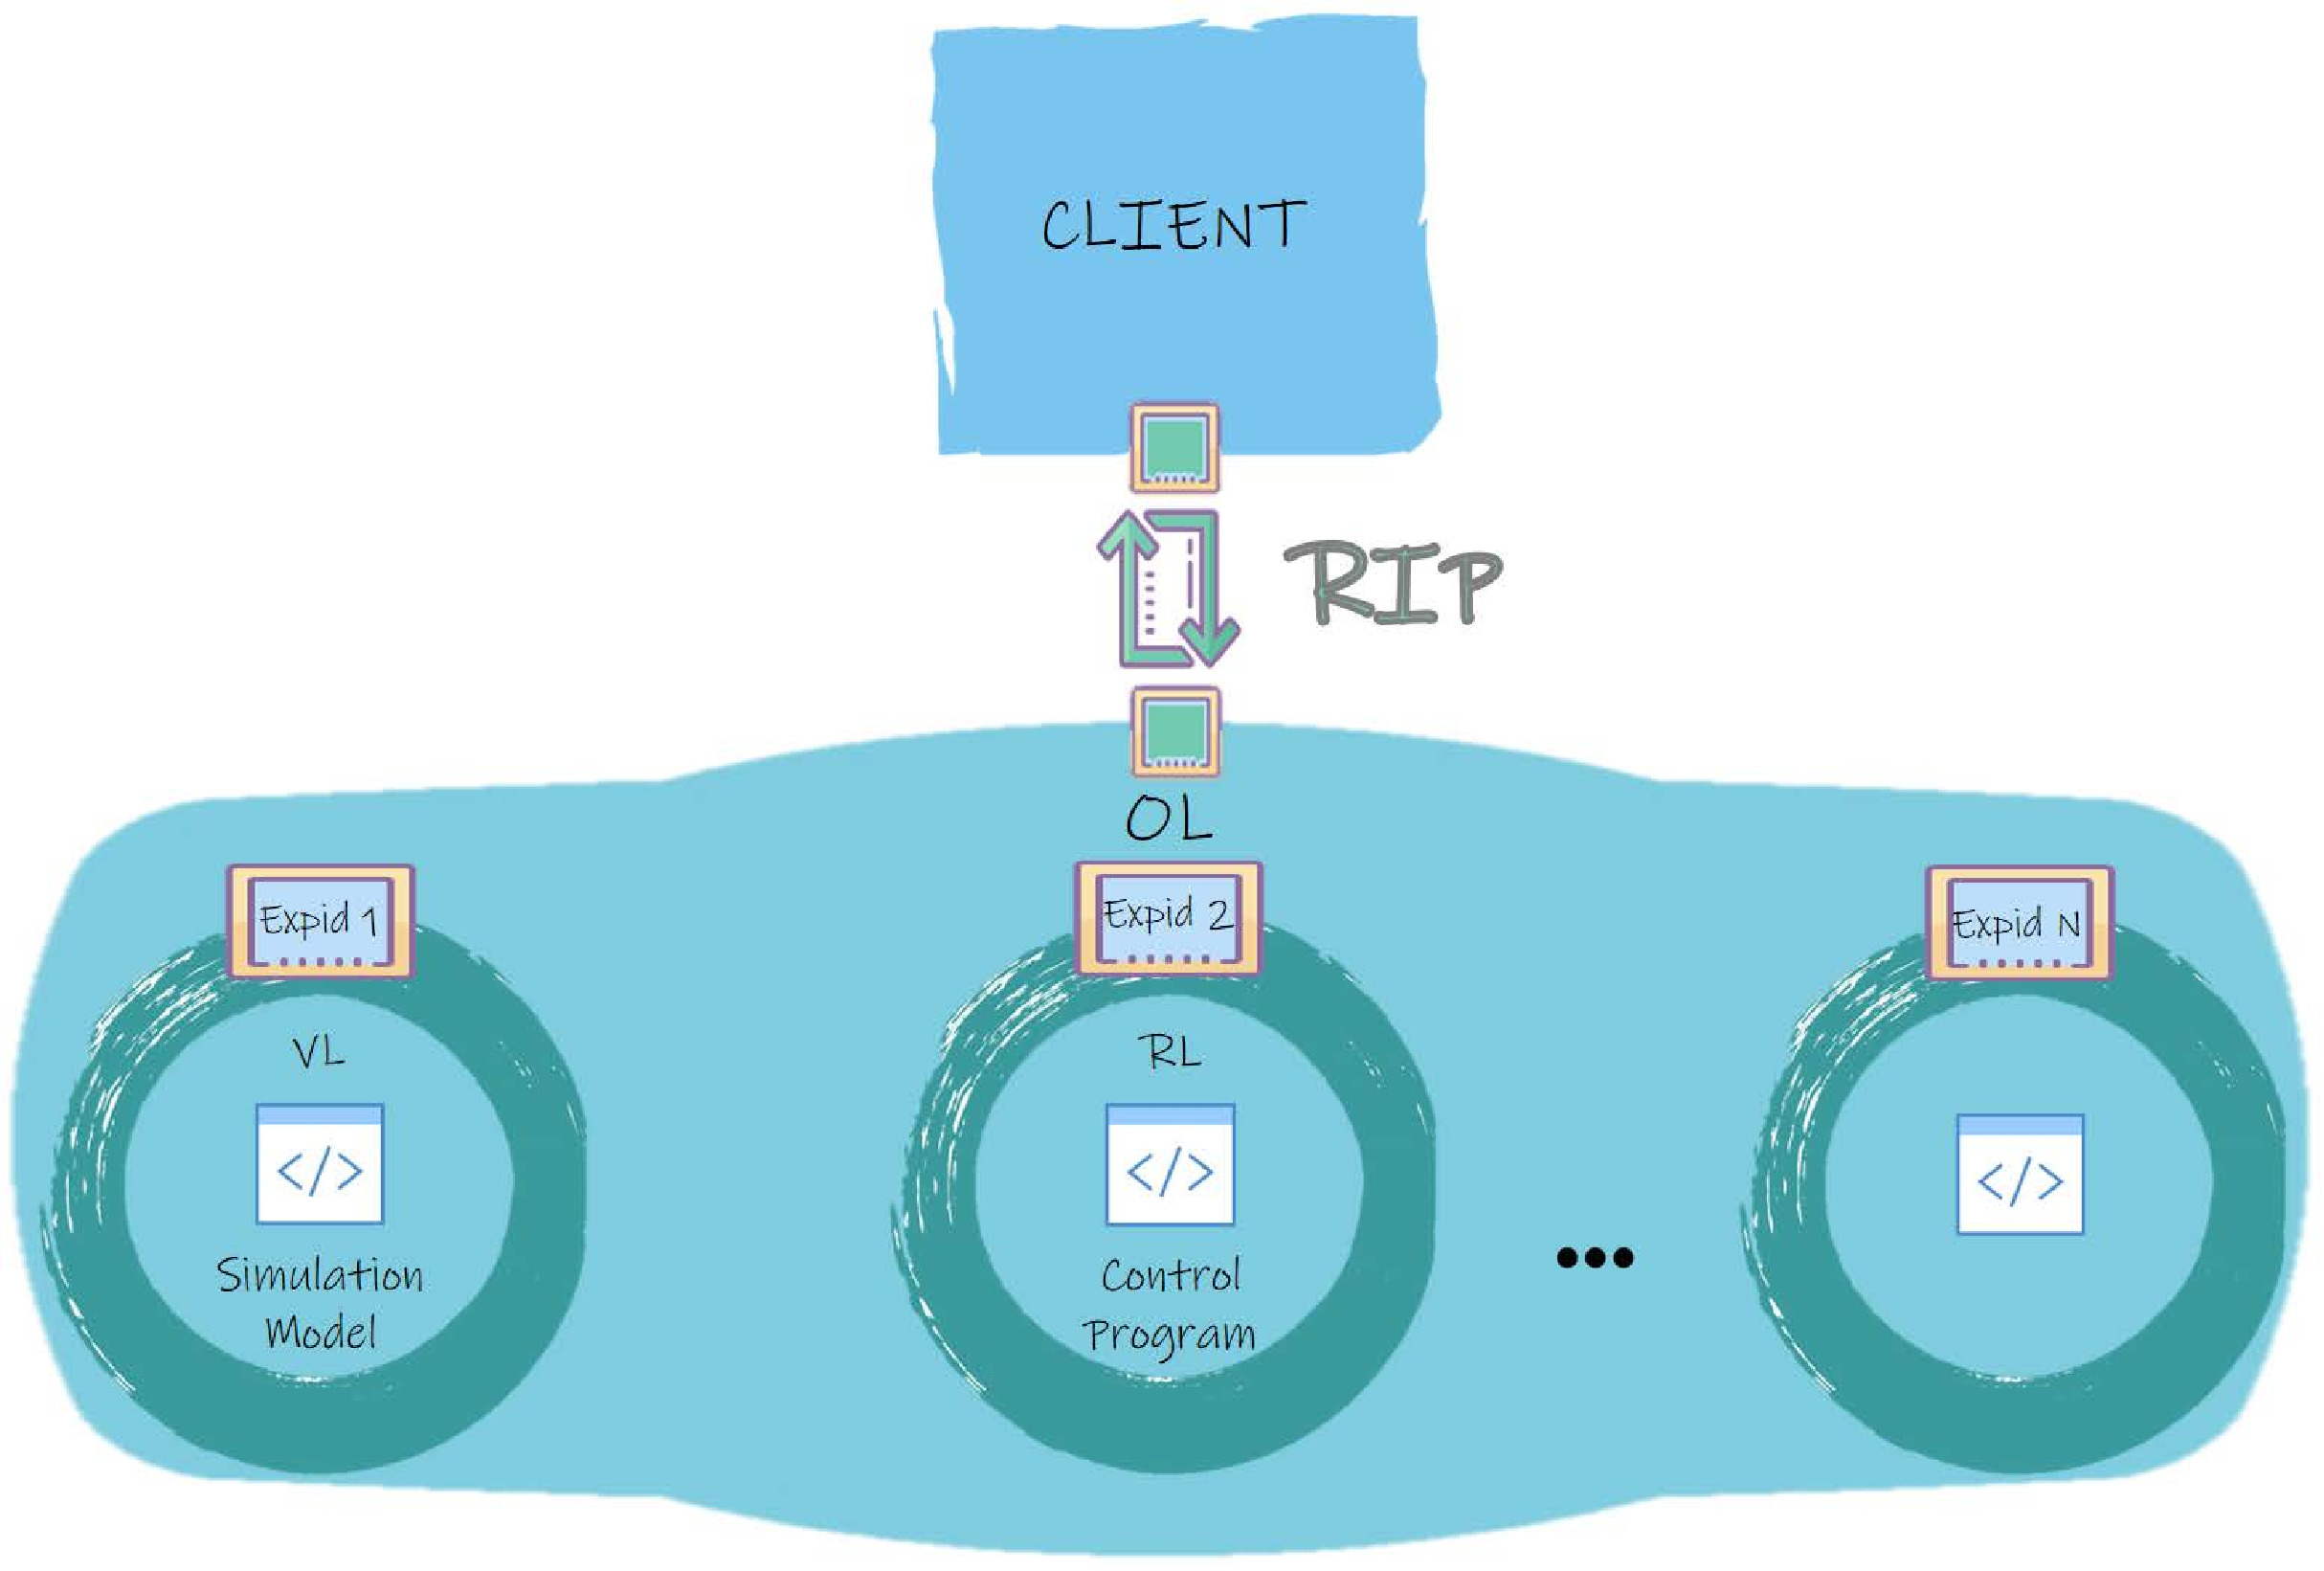
\includegraphics[width=0.75\textwidth]{images/Client-RIP-OL.pdf}
\caption{RIP protocol is used by a RIP client and a RIP server to communicate both. The RIP server is implemented in an OL and the RIP client is implemented in a web browser application.}
\label{fig:Client-RIP-OL}
\end{figure}


\chapter{Overall Description}
\label{Overall Description}

\section{Protocol Perspective}
The protocol is an open source, under the GNU general Public License. It is a communication protocol to be used in the client-server model, especially designed for OLs in which the client runs within a web browser. RIP provides a simple mechanism for users and client machines/programs to acquire information about the lab \textit{experiences} defined in the server and about each \textit{experience's} inputs and outputs. The protocol also defines methods for reading and writing the values of these inputs and outputs, respectively.

\begin{figure}[b!]
\centering
\includegraphics[width=0.5\textwidth]{images/RIPTechnologies.pdf}
\caption{RIP is based on POST and GET HTTP methods and on the JSON-RPC format.}
\label{fig:RIP_Technologies}
\end{figure}

The main features of RIP are the following:

\begin{enumerate}
    \item Defining \textit{experiences} on the OL.
    \item Obtaining meta-data related to each defined \textit{experience}.
    \item Obtaining a list of readable and writable variables for each \textit{experience}.
    \item Obtaining a list of methods to read and write variables in each \textit{experience}.
    \item Invoking methods to read and write variables in each \textit{experience}.
    \item Defining server events to send data either periodically or based on any other triggering condition defined in an \textit{experience}.
    \item Subscribing a client to any server event declared in an \textit{experience}.
\end{enumerate}

RIP is based on two cornerstones: POST and GET methods for the communications transport and JSON-RPC for formatting messages. POST and GET are HTTP methods, which, in turn, is based on TCP communications. On the other hand, JSON-RPC is based on the JSON format. Figure \ref{fig:RIP_Technologies} represents these ideas.

Communication between two software entities is possible when they talk the same protocol. Therefore, a RIP implementation is needed in both the client and the server.

\subsection{Server Implementation Perspective}
Figure \ref{fig:RIP_Architecture} depicts the architecture of a \emph{RIP Server} that implements the RIP protocol. To sum it up, there are three functional subsystems: the \emph{Web Server}, that handles client connections, user sessions, etc., the \emph{Command Interpreter}, that speaks RIP, and the \emph{Executor}, that controls the execution of the laboratory \textit{control programs} or \textit{simulation models}.

\begin{figure}[b!]
\centering
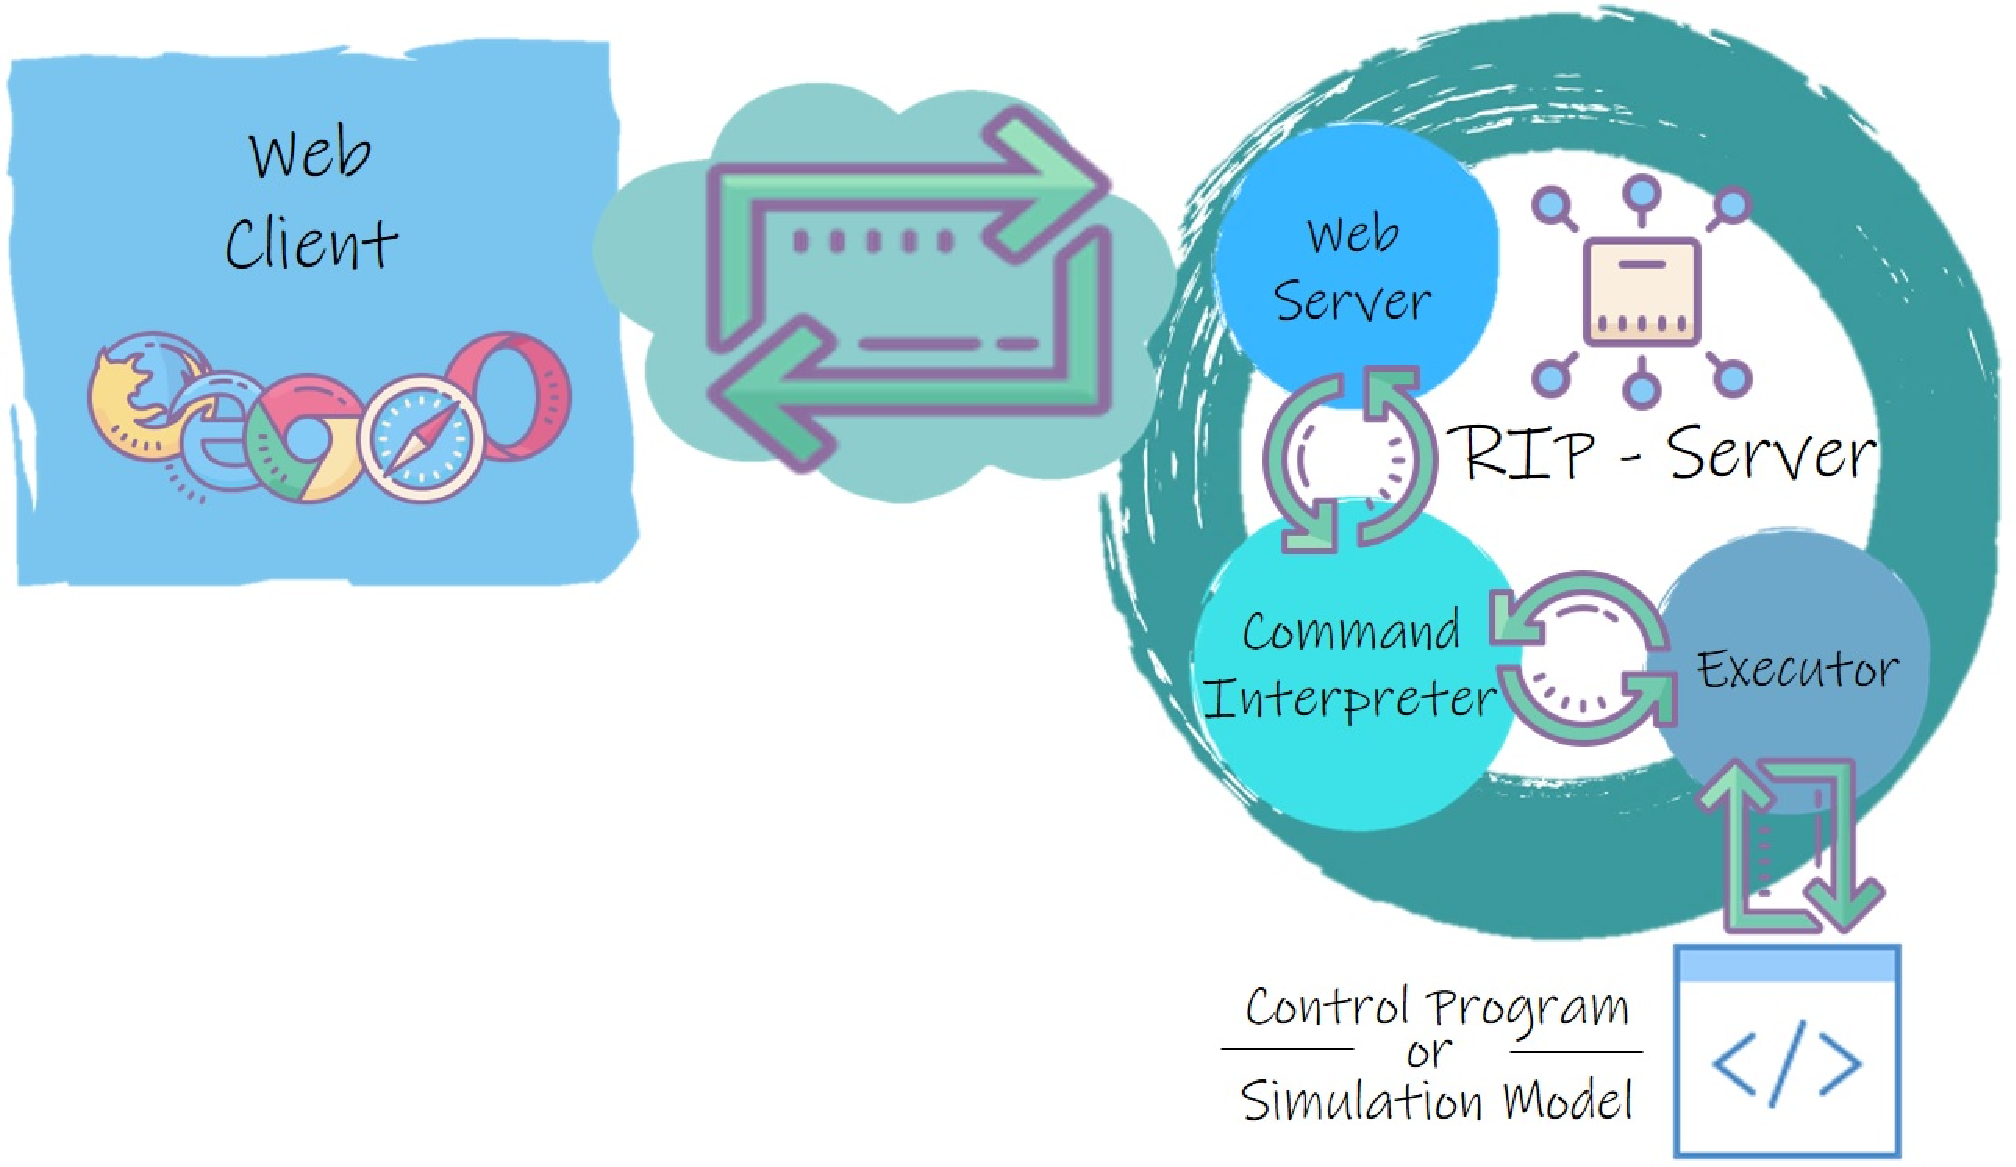
\includegraphics[width=0.75\textwidth]{images/RIPArchitecture.pdf}
\caption{Architectural view of a RIP Server}
\label{fig:RIP_Architecture}
\end{figure}

The \textit{Web Server} component admits (and handles in different ways) three types of requests: GET (used to retrieve \textit{experiences'} meta-data), SSE (used to get server-to-client data updates) and POST (used to send client-to-server updates or client-to-server requests for data updates). These different methods are each associated with the three basic cases of use, namely:

\begin{itemize}
    \item \emph{Meta-data} - A client, wanting to obtain information about the laboratory, launches an HTTP GET request to the URL associated with the laboratory. The RIP server responds with a JSON-RPC structure that informs the client, depending on the request's parameters, with one of the following:
    
    \begin{enumerate}
        \item General information about the OL: what are the \textit{experiences} defined and how they can be accessed.
        \item Detailed information of a particular \textit{experience} (when the request includes the {experience} id as a parameter).
    \end{enumerate}
    
    \item \emph{Observer} - A client, that desires to receive updates on the state of the plant, subscribes to an SSE event stream associated to the \textit{experience} of interest.
    
    \item \emph{Operator} - A client, wanting to act over the OL or to receive an update on demand, sends a POST request with the command codified as a RIP-JSON-RPC structure.
\end{itemize}

An \textit{experience} represents a lab activity associated with an OL. In the case of RLs, each \textit{experience} is implemented as a \textit{control program}, which in general is responsible of managing the physical connections with the hardware, safe measures, and any other functionality the lab designer has considered appropriate to include. In the case of VLs, each \textit{experience} is implemented as a \textit{simulation model} that represents a real system. The \textit{experience} abstraction is useful for two purposes: 1) to publish information about OLs in a standard and structured way and 2) to allow for hosting and running several different \textit{control programs} or \textit{simulation models} in the same computer.

\subsection{Client Implementation Perspective}
A RIP client must simply implement the required communication protocol methods (that is, POST, GET and SSE) with the appropriate format for reading and writing the messages content (that is, JSON-RPC) and the structure and functions defined by RIP (detailed in later sections).

\section{Protocol Functions (High-Level API)}
The functions defined and used in the protocol are divided in two types: internal and external.

The internal functions are private functions, used internally by RIP server implementations to communicate either with the \textit{simulation model} or the \textit{control program} used in the OL.

The external functions are client-side methods. These functions are used by the RIP clients to both get meta-data about the defined \textit{experiences} and to write and read data to and from the OL.

In this way, RIP servers must implement the internal functions, while RIP clients must implement the external functions (see Figure \ref{fig:Functions_Implementation}). Client-based methods of the external functions in a RIP client communicate with the \textit{Web Server} of a RIP server, get translated by the \textit{Command Interpreter} into a series of one or more internal functions, and are finally executed by the \textit{Executor} component (see Figure \ref{fig:RIP_Architecture}).

\begin{figure}[b!]
\centering
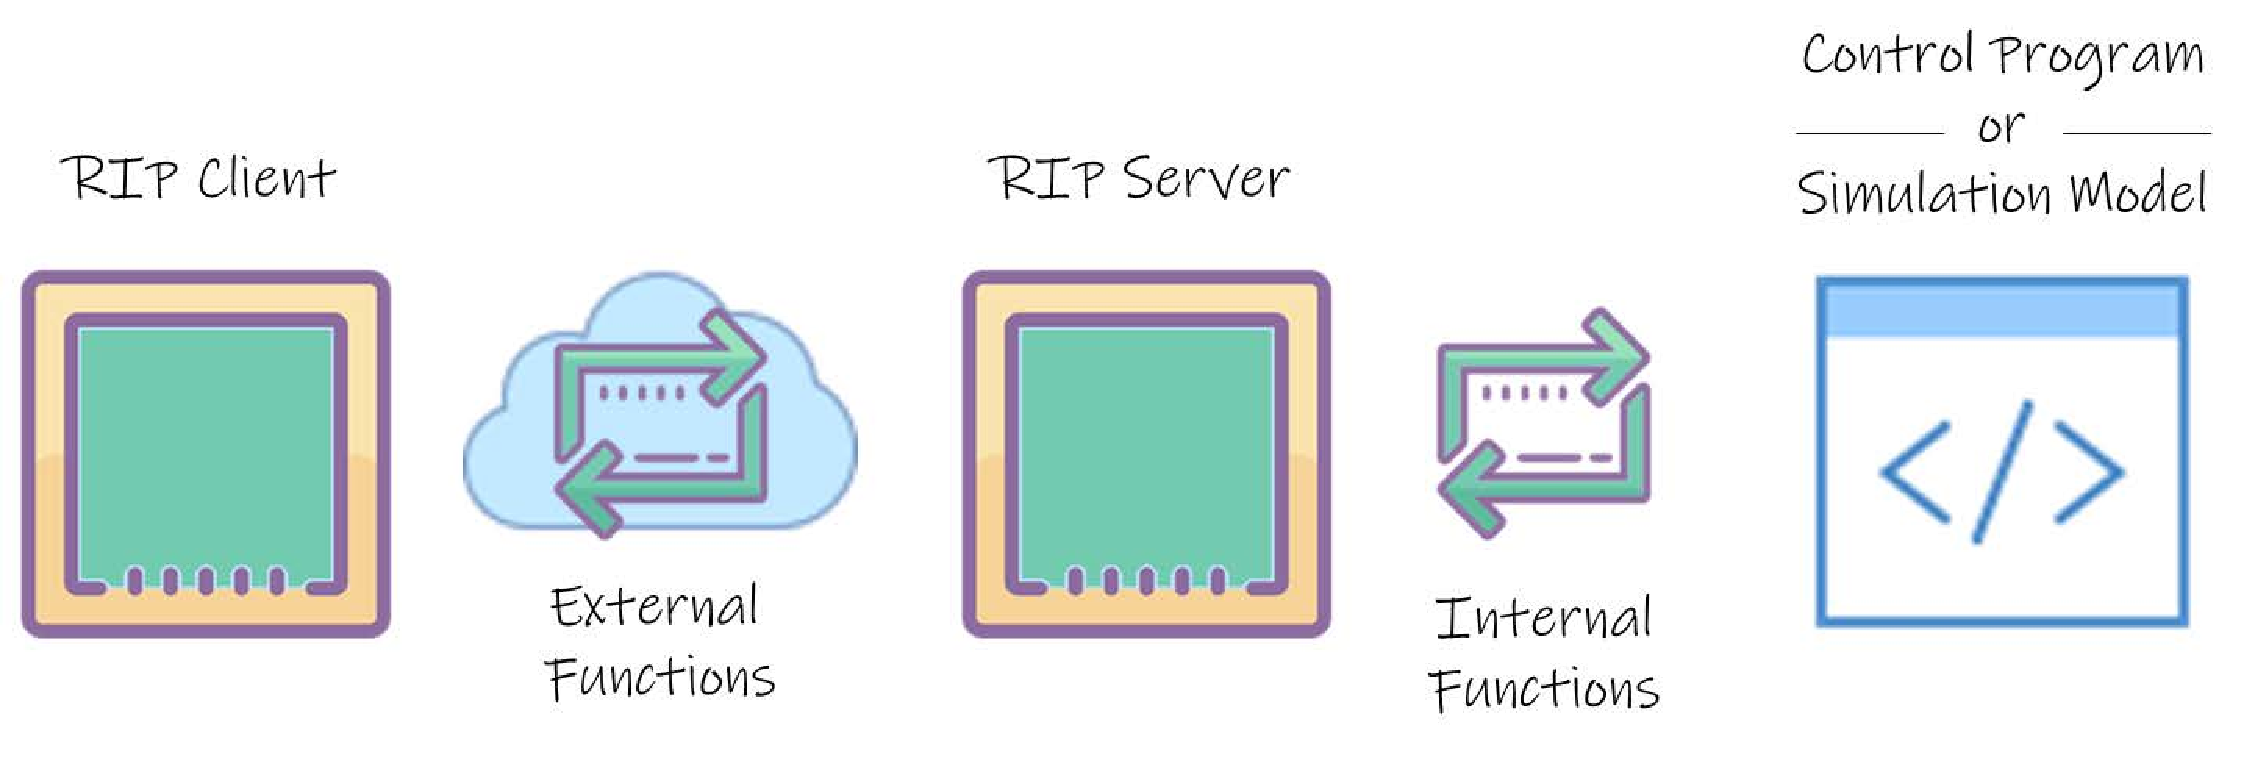
\includegraphics[width=0.75\textwidth]{images/FunctionsImplementation.pdf}
\caption{Internal and external functions implementation in RIP clients and servers}
\label{fig:Functions_Implementation}
\end{figure}

\subsection{Internal Functions}
\label{sec:Internal_Functions}
The list of internal functions a RIP server must implement is:

\begin{enumerate}
    \item \textit{info}  $=$ \textbf{basicInfo}(): Returns the list of \textit{experiences} defined in the OL and meta-data information about the method that can be used to retrieve more information about a particular \textit{experience}.
    \item \textit{info}  $=$ \textbf{experienceInfo}(\textit{expId}): Returns the list of variables defined in the \textit{control program} or \textit{simulation model} associated to the \textit{experience} defined by \textit{expId}, meta-data related to such \textit{experience} and information about the methods that can be used to communicate with the OL.
    \item \textit{readablelist}, \textit{writablelist}  $=$ \textbf{open}(\textit{expId}): Returns the list of readable and writable variables (in two different variables) defined in the \textit{experience} associated to the input \textit{expId} parameter.
    \item \textbf{close}(\textit{expId}): Closes the control program (if it is a RL) or the simulation model (if it is a VL) of the OL \textit{experience} defined by the input \textit{expId} parameter.
    \item \textbf{start}(\textit{expId}): Starts the execution of the \textit{control program} or \textit{simulation model} associated to the OL \textit{experience} defined by the input \textit{expId} parameter by: first, opening it and second, running it.
    \item \textbf{run}(\textit{expId}): Runs the \textit{control program} or \textit{simulation model} associated to the OL \textit{experience} defined by the input \textit{expId} parameter.
    \item \textbf{stop}(\textit{expId}): Stops the execution of the \textit{control program} or \textit{simulation model} associated to the OL \textit{experience} defined by the input \textit{expId} parameter.
    \item \textit{readVariableNames}, \textit{readVariableValues} $=$ \textbf{get}(\textit{expId}, \textit{variableNames}): Retrieves the current values of the variables (\textit{readVariableValues}) specified by the \textit{variableNames} input parameter. For this to happen, these variables must exist in the \textit{control program} or \textit{simulation model} associated to the \textit{experience} defined by the \textit{expId} input parameter. When the \textbf{get()} method is called, \textit{readVariableNames} contains only the names of the variables that were successfully read, not all requested ones in \textit{variableNames}.
    \item \textbf{set}(\textit{expId}, \textit{variableNames}, \textit{variableValues}): Writes the received values (\textit{variableValues}) in the specified variables (\textit{variableNames}) of the appropiate OL \textit{experience}. For this to happen, these variables must exist in the \textit{control program} or \textit{simulation model} associated to the (\textit{expId}) input parameter.
\end{enumerate}

\subsection{External Functions}
\label{sec:External_Functions}
The list of external functions a RIP client must implement is:

\begin{enumerate}
    \item \textit{result} $=$ \textbf{info}(\textit{callback}, \textit{expId} $=$ null): Retrieves the meta-data information about the \textit{experience} defined by the input \textit{expId} parameter. This parameter is optional and if it is not specified, the method then returns meta-data information about all the \textit{experiences} defined.
    \item \textbf{connect}(\textit{expId}, \textit{callback}): Connects to an \textit{experience} defined by the input \textit{expId} parameter and establishes connection to the SSE to start receiving server data updates.
    \item \textbf{set}(\textit{variableNames}, \textit{variableValues}, \textit{callback}, \textit{expId}): Writes the received values (\textit{variableValues}) in the specified variables (\textit{variableNames}) of the appropiate OL \textit{experience}. For this to happen, these variables must exist in the \textit{control program} or \textit{simulation model} associated to the (\textit{expId}) input parameter.
    \item \textit{result} $=$ \textbf{get}(\textit{variableNames}, \textit{callback}, \textit{expId}): Retrieves the current values of the variables (\textit{readVariableValues}) specified by the \textit{variableNames} input parameter. For this to happen, these variables must exist in the \textit{control program} or \textit{simulation model} associated to the \textit{experience} defined by the \textit{expId} input parameter.
\end{enumerate}

Where:

Variables \textit{variableNames} and \textit{variableValues} are arrays of text. For example: \textit{variableNames} $=$ ["x", "y", ...], \textit{variableValues} $=$ ["10", "a", ...].

At the moment, only numbers, text and booleans are supported as valid types for \textit{variableValues} and \textit{readVariableValues} in the \textbf{set}() and \textbf{get}() methods, respectively.

Sections \ref{sec:User_Doc} and \ref{sec:Developer_Doc} give more information about the external and internal functions, respectively.

\section{Protocol Communication Methods (Low-Level API)}
Three HTTP communication methods are available in RIP for communicating the client with the server:

\begin{enumerate}
    \item \textbf{GET} - To obtain OL meta-data. A RIP server must implement a web service endpoint at \url{BaseURL:port/RIP} for attending these requests.
    \item \textbf{POST} - To send client-to-server requests for (i) writing OL variables' values and (ii) reading OL variables' values. A RIP server must implement a web service endpoint at \url{BaseURL:port/RIP/POST} for attending these requests.
    \item \textbf{SSE} - To subscribe the client to data streams so that it receives server-to-client OL variables' values updates. A RIP server must implement a web service endpoint at \url{BaseURL:port/RIP/SSE} for attending these requests.
\end{enumerate}

Table \ref{tab:low-high-levels-correspondence} shows the correspondence between the external protocol functions of the high-level API and the HTTP methods of the low-level API. The right column also indicates the RIP's web server endpoint to which each of the methods and functions communicate with. A representation of these same ideas is shown in Figure \ref{fig:client-server-funtions-correspondence}. While they should, not all internal functions are represented in the Figure; only six out of nine appear in it.

\begin{table}[]
    \centering
    \begin{tabular}{c|c|c}
        \hline
        & \\RIP client function (High-Level API) & HTTP Method (Low-Level API) & Web server endpoint \\
        \hline
        & \\info(callback), info(callback, expId) & GET & /BaseURL:port/RIP \\
        \hline
        & \\set(variableNames, variableValues, callback, expId), & POST & /BaseURL:port/RIP/POST
          \\get(variableNames, expId) &  & \\
        \hline
        & \\connect(expId, callback) & SSE & /BaseURL:port/RIP/SSE \\
        \hline
    \end{tabular}
    \caption{Correspondence between RIP external functions, HTTP methods and RIP's web server endpoints}
    \label{tab:low-high-levels-correspondence}
\end{table}

Section \ref{sec:Developer_Doc} gives more information about the use of these HTTP methods in RIP's low-level API.

\section{Operating Environment}
RIP uses only HTTP methods for the communication. Therefore, it works in any major web browser. However, RIP also relies on the use of SSEs, which, up to date, are not supported by Microsoft Internet Explorer nor Microsoft Edge. Nevertheless, there are numerous poly-fill solutions for implementing SSE so that they work on these browsers that do not support them natively.

\section{Design and Implementation Constraints}
RIP is designed to only use pure HTTP methods on purpose, with the aim of guaranteeing its correct functioning from web browsers. Therefore, the only hard implementation constraint is that HTTP is used for implementing RIP communications.

\begin{figure}
\centering
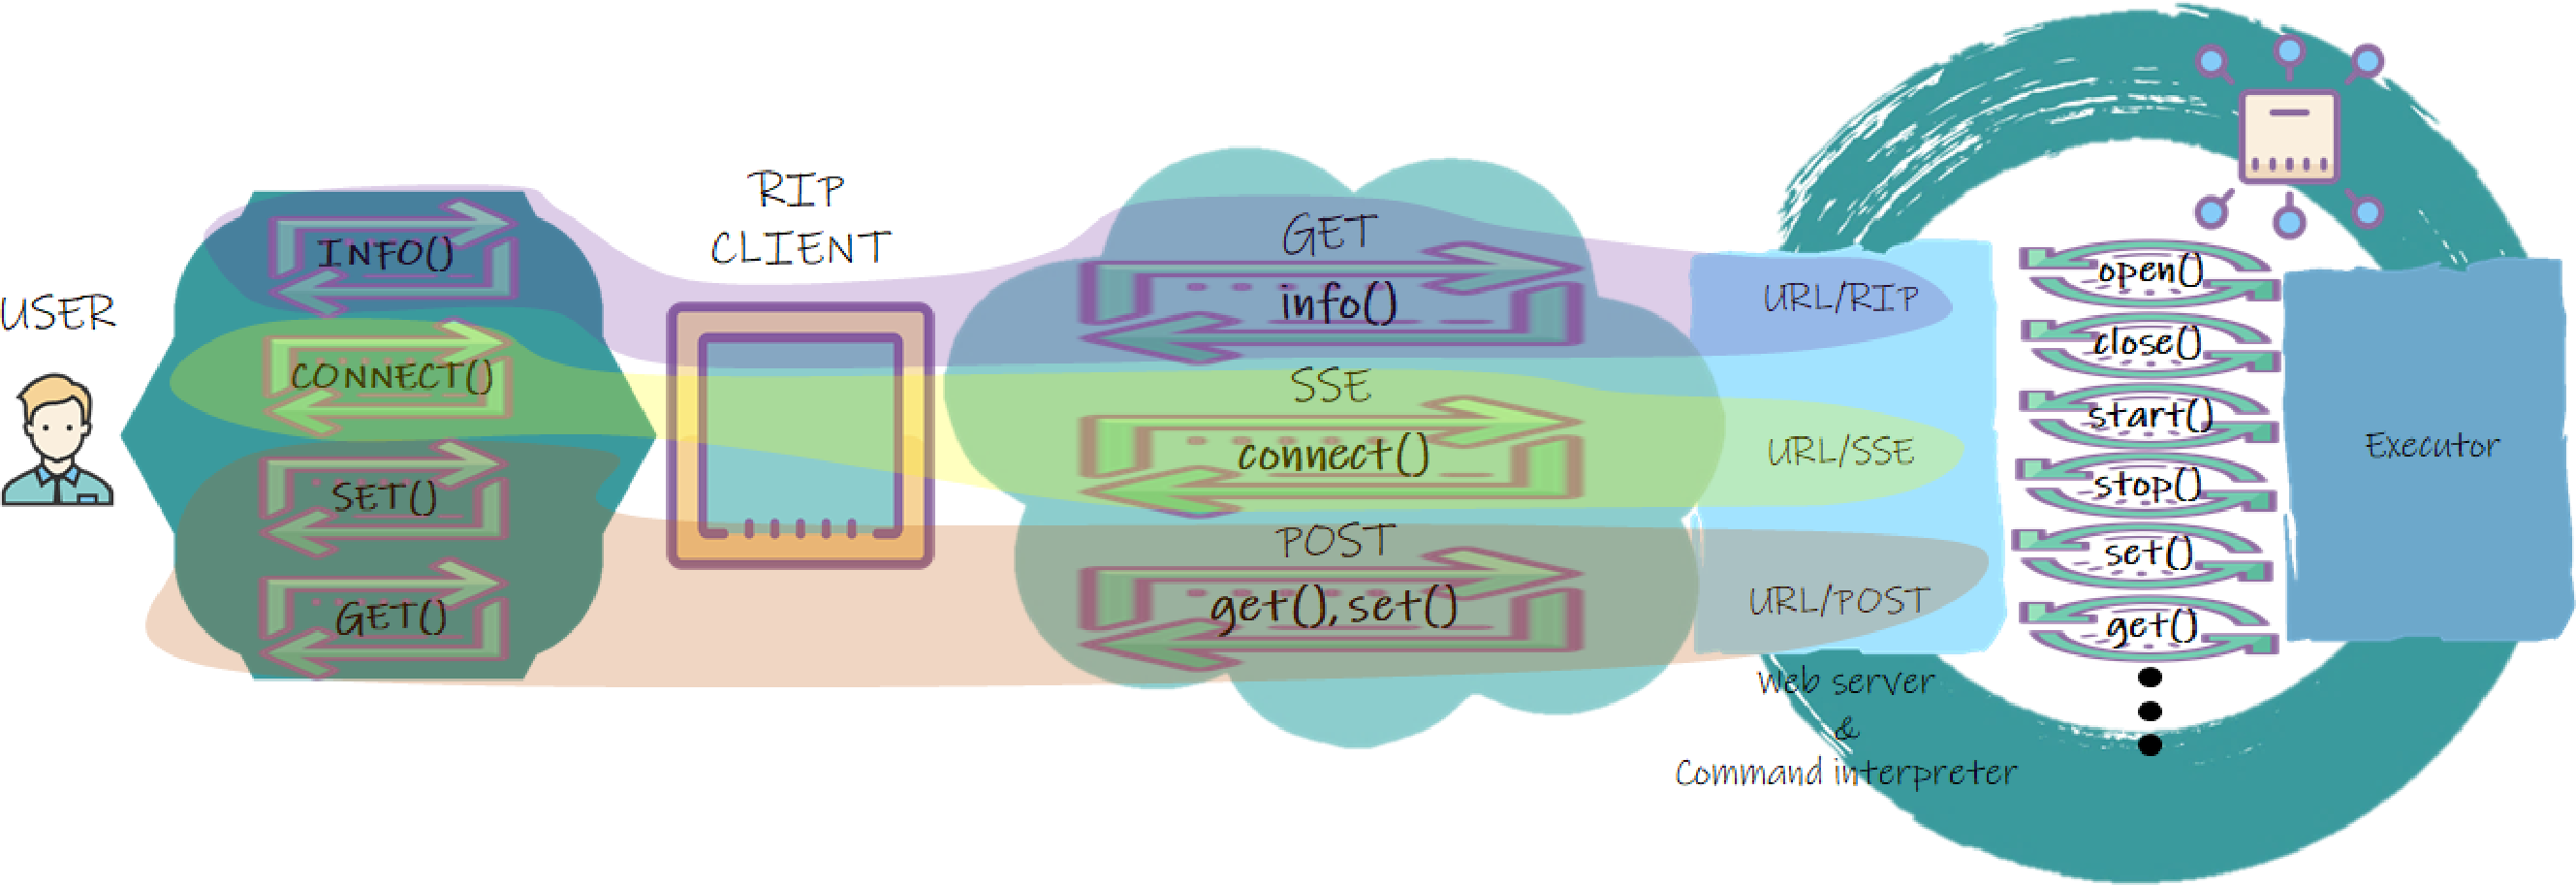
\includegraphics[width=\textwidth]{images/Correspondence.pdf}
\caption{Illustration of the existing correspondence between RIP functions, HTTP methods and RIP's web server endpoints}
\label{fig:client-server-funtions-correspondence}
\end{figure}

\section{Assumptions and Dependencies}
RIP depends solely on the use of HTTP POST and GET methods and on the JSON format for exchanging data. 
A common and easy way of implementing RIP in web clients is through the use of the EventSource object \cite{sse} (for the SSEs) and the XMLHttpRequest object \cite{xhr} or the Fetch API \cite{fetch} (for the POST messages), which are both supported by all major web browsers. Still, implementations without the use of such APIs are possible, just more laborious. 

RIP server implementations may differ a lot depending on the language used to make the implementation, and so do their possible dependencies.

\section{User Documentation}
\label{sec:User_Doc}
This section provides a deeper insight on the external functions of the high-level API from a final user point of view. This is the only knowledge required by such a user to use a RIP client implementation to communicate with an OL running a RIP server.

A RIP client must implement a class with the methods described in Section \ref{sec:External_Functions}. Next, detailed information of each of them is given. This information includes a description of: 1) the method itself, 2) its input parameters and 3) the result returned by the method. All methods have a \textit{callback} parameter; a function to be called after the method completes its tasks.

\subsection{Method info}
This method has two input parameters: \textit{callback} and  \textit{expId}. It can be called with or without the \textit{expId} parameter.

When called without this parameter, \textbf{info}() returns meta-data with the list of experience identifiers associated to all \textit{experiences} defined in the OL. It also returns more information about the low-level API method call for retrieving meta-data.

When called with the \textit{expId} parameter, \textbf{info}(\textit{expId}) returns meta-data of the referenced \textit{experience}.

The result returned by this method is a string in JSON format containing information about the experience defined in the RIP server with name \textit{expId}. The structure and content of this string depends on whether the method is called with or without the \textit{expId} parameter. In any case, the result is described in detail in section \ref{sec:info}.

The way to call it is:

\textit{result} $=$ \textbf{info}(\textit{callback}, \textit{expId} $=$ null)

\subsection{Method connect}
This method has two input parameters: \textit{expId} and \textit{callback}.

When this method is called, the client connects to an SSE in the RIP server to: 1) control the user session in the server and 2) receive updates of the variables value in the \textit{experience} defined by \textit{expId}.

This method returns nothing and the way to call it is: 

\textbf{connect}(\textit{expId}, \textit{callback})

\subsection{Method set}
This method has four input parameters: \textit{variableNames} and \textit{variableValues}, \textit{callback} and \textit{expId}, .

When this method is called, the values specified in \textit{variableValues} are assigned to the \textit{control program's} or \textit{simulation model's} variables named as the strings in \textit{variableNames}. The \textit{control program} or \textit{simulation model} is determined with the \textit{expId} parameter. 

This method returns nothing and the way to call it is: \textbf{set}(\textit{variableNames}, \textit{variableValues}, \textit{callback}, \textit{expId})

\subsection{Method get}
This method has three input parameters: \textit{variableNames}, \textit{callback} and \textit{expId}.

When this method is called, the values of the \textit{control program's} or \textit{simulation model's} variables named as the strings in \textit{variableNames} are read and returned. The \textit{control program} or \textit{simulation model} is determined with the \textit{expId} parameter.

The result returned by this method is a mixed array with the current values of the \textit{control program's} or \textit{simulation model's} variables specified in the \textit{variableNames} input parameter.

The way to call it is:

\textit{result} $=$ \textbf{get}(\textit{variableNames}, \textit{callback}, \textit{expId})

\section{Developer Documentation}
\label{sec:Developer_Doc}
This section provides more details on the internal functions of the high-level API and on the low-level API, which represents the knowledge required to either implement a new RIP client or a new RIP server, or to modify existing ones.

\subsection{Internal Functions of the High-Level API}
The High-Level API internal functions are run in the RIP server upon the reception of a GET or POST message, or when an SSE connection is established, mostly. Table \ref{tab:internal-external-correspondence} shows the correspondence between the external function called by the client and the internal function executed at the server.

\begin{table}[b!]
    \centering
    \begin{tabular}{|c|c|}
        \hline
        & \\RIP (client) external function & RIP (server) internal functions \\
        \hline
        & \\info(callback) & basicInfo() \\
        \hline
        & \\info(callback, expId) & experienceInfo() \\
        \hline
        & \\connect(expId, callback) & 1. - start(), 2. - get() \\
        \hline
        & \\set(variableNames, variableValues, callback, expId) & set() \\
        \hline
        & \\get(variableNames, callback, expId) & get() \\
        \hline
    \end{tabular}
    \caption{Correspondence between RIP external functions and RIP internal functions}
    \label{tab:internal-external-correspondence}
\end{table}

However, the execution of some internal functions are not fired due to the reception of an external function in the RIP server. On the contrary, some internal functions are run when a client disconnection is detected (that's the case of the \textit{stop()} and \textit{close()} methods), or when other internal functions are called (\textit{open()} and \textit{run()} methods). Table summarizes this information.

\begin{table}[b!]
    \centering
    \begin{tabular}{|c|c|}
        \hline
        & \\Trigger condition & Executed RIP (server) internal functions \\
        \hline
        & \\experienceInfo() is run & 1. - [open()], 2. - get(), 3. - [close()] \\
        \hline
        & \\start() is run & 1 . - [open()], 2. - [run()] \\
        \hline
        & \\Client disconnects & 1. - [stop()], 2. - [close()] \\
        \hline
    \end{tabular}
    \caption{Triggering conditions and fired internal methods}
    \label{tab:trigerring-internal-correspondence}
\end{table}

Functions between brackets in Table \ref{tab:trigerring-internal-correspondence} are not necessarily run, and only get executed when needed.

As can be seen in Tables \ref{tab:internal-external-correspondence} and \ref{tab:trigerring-internal-correspondence}, the \textit{get()} internal function can be either run upon a client function reception (\textit{connect(expId)} and \textit{get(expId, variableNames)}) or due to the execution of the \textit{experienceInfo()} internal method. 

Each method returns an error indicator when the operation is not completed successfully.

\subsubsection{Method basicInfo}
This method is called only when the RIP server receives an HTTP message from a client with the \textit{info} method and no parameters.

It returns a list of \textit{experiences} defined in the OL and meta-data information about the GET HTTP RIP method described in previous sections to get meta-data.

\subsubsection{Method experienceInfo}
This method is called only when the RIP server receives an HTTP message from a client with the \textit{info} method and the \textit{expId} parameter.

It returns meta-data information about the \textit{experience} and the available HTTP RIP methods described in previous sections to communicate with the OL.

\subsubsection{Method start}
This method is called only when the RIP server receives an HTTP message from a client with the \textit{connect} method and the \textit{expId} parameter.

It runs (when needed) two internal functions in order: first, \textit{open()} and second, \textit{run()}, to open and run the \textit{control program} or \textit{simulation model} associated to the experience, respectively.

\subsubsection{Method open}
This method is run only when either the experienceInfo() or the start() methods are called in the RIP server and there are no other clients using the associated \textit{experience}, which means the corresponding \textit{control program} or \textit{simulation model} is closed.

It opens the \textit{control program} or \textit{simulation model} associated to the experience.

\subsubsection{Method close}
This method is run either when a client disconnection is produced, with the objective of closing the \textit{control program} or \textit{simulations model} that was open to attend the client requests, or when the experienceInfo() method is called and there are no other clients using the associated \textit{experience}.

It closes the \textit{control program} or \textit{simulation model} associated to the experience.

\subsubsection{Method run}
This method is run only when either the start() method is called in the RIP server and there are no other clients using the associated \textit{experience}, which means the corresponding \textit{control program} or \textit{simulation model} is not currently running.

It runs the \textit{control program} or \textit{simulation model} associated to the experience.

\subsubsection{Method stop}
This method is only run when a client disconnection is produced, with the objective of stopping the execution of the \textit{control program}, or \textit{simulations model} that was running to attend the client requests. 

It stops the \textit{control program} or \textit{simulation model} associated to the experience.

\subsubsection{Method get}
This method is called only when the RIP server receives an HTTP message from a client either with the \textit{get} method and the \textit{expId} and \textit{variableNames} parameters or with the \textit{connect} method method and the \textit{expId} parameter. In the first case, this method is called only once. In the second, as an SSE communication is established, the method is called receptively, depending on the events defined in the RIP server.

It returns the list of current values of the variables defined in the \textit{control program} or {simulation model} and the names of the read variables.

\subsubsection{Method set}
This method is called only when the RIP server receives an HTTP message from a client with the \textit{set} method and the \textit{expId}, \textit{variableNames} and \textit{variableValues} parameters.

It writes the values received in the specified variables of the appropriate OL \textit{experience}.

\subsection{Low-Level API}
Each external method from the High-Level API is implemented with an HTTP method that follows the Low-Level API. The nature and structure of the HTTP messages that must be built by each High-Level API method, the RIP server endpoint to which it must connect, and the result returned by the RIP server to each of these messages is detailed in this section.

For the sake of clarity, each method also includes an example. The relevant parameters for this example can be found in Table \ref{tab:low-level-example}.

\begin{table}[]
    \centering
    \begin{tabular}{|c|c|}
        \hline
         & \\Parameter & Value \\
         \hline
         & \\Protocol & http \\
         \hline
         & \\BaseURL & 10.192.38.56 \\
        \hline
        & \\Communication port & 8080 \\
        \hline
         & \\Declared experiences & Test1, Test2 \\
        \hline
         & \\Declared inputs in \textit{control program} & stringin, intin, doublein, booleanin
         \\or \textit{simulation model} for Test1 & \\
        \hline
        & \\Declared outputs in \textit{control program} & stringout, intout, doubleout, booleanout
          \\or \textit{simulation model} for Test1 & \\
        \hline
    \end{tabular}
    \caption{Relevant parameters for the examples.}
    \label{tab:low-level-example}
\end{table}

\subsubsection{Method info - GET}
\label{sec:info}
The \textit{info(callback)} RIP client method sends a GET request to \url{http(s)://BaseURL:port/RIP}, while \textit{info(callback, expIdValue)} does the same with \url{http(s)://BaseURL:port/RIP?expId=expIdValue}.

The result of calling this method without the \textit{expId} input parameter is a JSON object containing one single top-level member:

\begin{myEnumerate}
    \item \textbf{experiences}: A JSON object with the following top-level members:
    \begin{myEnumerate}
        \item \textbf{list}: An array of JSON objects, each of which contains one single top-level member:
        \begin{myEnumerate}
            \item \textbf{id}: A string with the experience identifier (expId) that is unmistakably related to one and only one \textit{experience} defined in the OL.
        \end{myEnumerate}
        \item \textbf{methods}: An array of JSON objects, each of which contains the following top-level members:
        \begin{myEnumerate}
            \item \textbf{url}: A string with the URL to call the method.
            \item \textbf{type}: A string specifying the HTTP method to use.
            \item \textbf{description}: A string describing the method.
            \item \textbf{params}: An array of JSON objects detailing the required and optional parameters for the method:
            \begin{myEnumerate}
                \item \textbf{name}: A string with the name of the parameter
                \item \textbf{required}: A string ("yes" or "no") specifying whether the parameter is required ("yes") or optional ("no").
                \item \textbf{location}: A string referencing the location for the parameter ("query", "header" or "body").
                \item \textbf{value}: [Optional] A string with the required value for the parameter.
                \item \textbf{type}: [Optional] A string detailing the type of the parameter.
                \item \textbf{elements}: [Optional] An array of JSON objects with the following top-level members:
                \begin{myEnumerate}
                    \item \textbf{description}: A string with a description of the parameter element.
                    \item \textbf{type}: A string specifying the type of the parameter element.
                    \item \textbf{subtype}: [Optional] A string detailing the type of the elements inside an array parameter element when they are all of the same type.
                \end{myEnumerate}
                \item \textbf{subtype}: [Optional] A string detailing the type of the elements inside an array parameter when they are all of the same type.
            \end{myEnumerate}
            \item \textbf{returns}: A string with the MIME-type of the method's result.
            \item \textbf{example}: A JSON object with the following top-level members:
            \begin{myEnumerate}
                    \item \textbf{url}: A string with the URL to call the method.
                    \item \textbf{headers}:[Optional] A JSON object with the parameters to be placed on the HTTP request headers with as many top-level members as headers are set:
                    \begin{myEnumerate}
                        \item \textbf{HeaderName}: HeaderValue
                    \end{myEnumerate}
                    \item \textbf{body}: [Optional] A JSON object with the parameters to be placed on the HTTP request body and with the following top-level members:
                    \begin{myEnumerate}
                        \item \textbf{jsonrpc}: "2.0"
                        \item \textbf{method}: A string with the RIP method to invoke ("get", "set" or "connect"). % "start" or "stop").
                        \item \textbf{params}: An array with the following elements:
                        \begin{myEnumerate}
                            \item \textbf{expId}: A string with the \textit{eperience} identifier.
                            \item \textbf{variableNames}: An array of strings in which each element has the name of a variable in the \textit{control program} or in the \textit{simulation model}.
                            \item \textbf{variableValues}: [Optional] An array of strings with the values to be written in the variables specified in the \textit{variableNames} member, following the same order.
                        \end{myEnumerate}
                        \item \textbf{id}: A string with a number that indicates how many request have been sent till now, including this one.
                    \end{myEnumerate}
            \end{myEnumerate}
        \end{myEnumerate}
    \end{myEnumerate}
\end{myEnumerate}

\textbf{\underline{Example:}}

\textit{Request:}

The \textit{info(callback)} RIP client method sends a GET request to: \url{http://10.192.38.56:8080/RIP}

\textit{Response:}

The RIP server responds to the GET message with the following body:

\begin{lstlisting}
{
  "experiences": {
    "list": [
              {
              "id": "Test1"
              },
              {
              "id": "Test2"
              }
            ],
    "methods": [
                  {
                  "url": "10.192.38.56:8080/RIP",
                  "type": "GET",
                  "description": "Retrieves information (variables and methods) of the experiences in the server",
                  "params": [
                               {
                               "name": "Accept",
                               "required": "no",
                               "location": "header",
                               "value": "application/json"
                               },
                               {
                               "name": "expId",
                               "required": "no",
                               "location": "query",
                               "type": "string" 
                               }
                            ],
                  "returns": "application/json",
                  "example": {
                             "url": "10.192.38.56:8080/RIP?expId=Test1"
                             }
                  }
               ]
    }
}
\end{lstlisting}

The result of calling this method with the \textit{expId} input parameter is a JSON object containing three top-level members:

\begin{myEnumerate}
    \item \textbf{info}: A JSON object with the following top-level members:
    \begin{myEnumerate}
        \item \textbf{name}: A string with the name given to the experience.
        \item \textbf{description}: A string with a description of the experience.
        \item \textbf{authors}: A string with the name of the authors of the experience, separated by commas.
        \item \textbf{keywords}: An array of strings, each with a keyword related to the experience.
    \end{myEnumerate}
    \item \textbf{readables}: A JSON object with the following top-level members:
    \begin{myEnumerate}
        \item \textbf{list}: An array of JSON objects with the following top-level members:
        \begin{myEnumerate}
            \item \textbf{name}: A string with the name of the variable.
            \item \textbf{description}: A string with a description of the variable.
            \item \textbf{type}: A string with the type of the variable: \textit{"string"}, \textit{"int"}, \textit{"float"} or \textit{"boolean"}.
            \item \textbf{min}: A string with the minimum value the variable can have. In case of boolean variables, \textit{"false"}; in case of string variables, \textit{""}; in any other case, any number in string format.
            \item \textbf{max}: A string with the minimum value the variable can have. In case of boolean variables, \textit{"true"}; in case of string variables, \textit{""}; in any other case, any number in string format.
            \item \textbf{precision}: A string with the minimum value the variable can have. In case of boolean or string variables, \textit{""}; in any other case, any number in string format.
        \end{myEnumerate}
        \item \textbf{methods}: EXACTLY AS the \textit{methods} top-level member from the \textit{experiences} JSON object returned by the \textit{info(callback)} method when called without the \textit{expId} parameter: an array of JSON objects, each of which contains the following top-level members:
        \begin{myEnumerate}
            \item \textbf{url}: A string with the URL to call the method.
            \item \textbf{type}: A string specifying the HTTP method to use.
            \item \textbf{description}: A string describing the method.
           \item \textbf{params}: An array of JSON objects detailing the required and optional parameters for the method:
            \begin{myEnumerate}
                \item \textbf{name}: A string with the name of the parameter
                \item \textbf{required}: A string ("yes" or "no") specifying whether the parameter is required ("yes") or optional ("no").
                \item \textbf{location}: A string referencing the location for the parameter ("header", "query" or "body").
                \item \textbf{value}: [Optional] A string with the required value for the parameter.
                \item \textbf{type}: [Optional] A string detailing the type of the parameter.
                \item \textbf{elements}: [Optional] An array of JSON objects with the following top-level members:
                \begin{myEnumerate}
                    \item \textbf{description}: A string with a description of the parameter element.
                    \item \textbf{type}: A string specifying the type of the parameter element.
                    \item \textbf{subtype}: [Optional] A string detailing the type of the elements inside an array parameter element when they are all of the same type.
                \end{myEnumerate}
                \item \textbf{subtype}: [Optional] A string detailing the type of the elements inside an array parameter when they are all of the same type.
            \end{myEnumerate}
            \item \textbf{returns}: A string with the MIME-type of the method's result.
            \item \textbf{example}: A JSON object with the following top-level members:
            \begin{myEnumerate}
                    \item \textbf{url}: A string with the URL to call the method.
                    \item \textbf{headers}:[Optional] A JSON object with the parameters to be placed on the HTTP request headers with as many top-level members as headers are set:
                    \begin{myEnumerate}
                        \item \textbf{HeaderName}: HeaderValue
                    \end{myEnumerate}
                    \item \textbf{body}: [Optional] A JSON object with the parameters to be placed on the HTTP request body and with the following top-level members:
                    \begin{myEnumerate}
                        \item \textbf{jsonrpc}: "2.0"
                        \item \textbf{method}: A string with the RIP method to invoke ("get", "set" or "connect"). %, "start" or "stop").
                        \item \textbf{params}: An array with the following elements:
                        \begin{myEnumerate}
                            \item \textbf{expId}: A string with the \textit{eperience} identifier.
                            \item \textbf{variableNames}: An array of strings in which each element has the name of a variable in the \textit{control program} or in the \textit{simulation model}.
                            \item \textbf{variableValues}: [Optional] An array of strings with the values to be written in the variables specified in the \textit{variableNames} member, following the same order.
                        \end{myEnumerate}
                        \item \textbf{id}: A string with a number that indicates how many request have been sent till now, including this one.
                    \end{myEnumerate}
            \end{myEnumerate}
        \end{myEnumerate}
    \end{myEnumerate}
    \item \textbf{writables}: A JSON object with the following top-level members:
    \begin{myEnumerate}
        \item \textbf{list}: EXACTLY AS the \textit{list} top-level member from \textit{readables}: an array of JSON objects with the following top-level members:
        \begin{myEnumerate}
            \item \textbf{name}: A string with the name of the variable.
            \item \textbf{description}: A string with a description of the variable.
            \item \textbf{type}: A string with the type of the variable: \textit{"string"}, \textit{"int"}, \textit{"float"} or \textit{"boolean"}.
            \item \textbf{min}: A string with the minimum value the variable can have. In case of boolean variables, \textit{"false"}; in case of string variables, \textit{""}; in any other case, any number in string format.
            \item \textbf{max}: A string with the minimum value the variable can have. In case of boolean variables, \textit{"true"}; in case of string variables, \textit{""}; in any other case, any number in string format.
            \item \textbf{precision}: A string with the minimum value the variable can have. In case of boolean or string variables, \textit{""}; in any other case, any number in string format.
        \end{myEnumerate}
        \item \textbf{methods}: EXACTLY AS the \textit{methods} top-level member from the \textit{experiences} JSON object returned by the \textit{info(callback)} method when called without the \textit{expId} parameter: an array of JSON objects, each of which contains the following top-level members:
        \begin{myEnumerate}
            \item \textbf{url}: A string with the URL to call the method.
            \item \textbf{type}: A string specifying the HTTP method to use.
            \item \textbf{description}: A string describing the method.
            \item \textbf{params}: An array of JSON objects detailing the required and optional parameters for the method:
            \begin{myEnumerate}
                \item \textbf{name}: A string with the name of the parameter
                \item \textbf{required}: A string ("yes" or "no") specifying whether the parameter is required ("yes") or optional ("no").
                \item \textbf{location}: A string referencing the location for the parameter ("header", "query" or "body").
                \item \textbf{value}: [Optional] A string with the required value for the parameter.
                \item \textbf{type}: [Optional] A string detailing the type of the parameter.
                \item \textbf{elements}: [Optional] An array of JSON objects with the following top-level members:
                \begin{myEnumerate}
                    \item \textbf{description}: A string with a description of the parameter element.
                    \item \textbf{type}: A string specifying the type of the parameter element.
                    \item \textbf{subtype}: [Optional] A string detailing the type of the elements inside an array parameter element when they are all of the same type.
                \end{myEnumerate}
                \item \textbf{subtype}: [Optional] A string detailing the type of the elements inside an array parameter when they are all of the same type.
            \end{myEnumerate}
            \item \textbf{returns}: A string with the MIME-type of the method's result.
            \item \textbf{example}: A JSON object with the following top-level members:
            \begin{myEnumerate}
                    \item \textbf{url}: A string with the URL to call the method.
                    \item \textbf{headers}:[Optional] A JSON object with the parameters to be placed on the HTTP request headers with as many top-level members as headers are set:
                    \begin{myEnumerate}
                        \item \textbf{HeaderName}: HeaderValue
                    \end{myEnumerate}
                    \item \textbf{body}: [Optional] A JSON object with the parameters to be placed on the HTTP request body and with the following top-level members:
                    \begin{myEnumerate}
                        \item \textbf{jsonrpc}: "2.0"
                        \item \textbf{method}: A string with the RIP method to invoke ("get", "set" or "connect"). %, "start" or "stop").
                        \item \textbf{params}: An array with the following elements:
                        \begin{myEnumerate}
                            \item \textbf{expId}: A string with the \textit{eperience} identifier.
                            \item \textbf{variableNames}: An array of strings in which each element has the name of a variable in the \textit{control program} or in the \textit{simulation model}.
                            \item \textbf{variableValues}: [Optional] An array of strings with the values to be written in the variables specified in the \textit{variableNames} member, following the same order.
                        \end{myEnumerate}
                        \item \textbf{id}: A string with a number that indicates how many request have been sent till now, including this one.
                    \end{myEnumerate}
            \end{myEnumerate}
        \end{myEnumerate}
    \end{myEnumerate}
\end{myEnumerate}

\textbf{\underline{Example:}}

\textit{Request:}

The \textit{info(callback, expId)} RIP client method sends a GET request to: \url{http://10.192.38.56:8080/RIP?expId=Test1}

\textit{Response:}

The RIP server responds to the GET message with the following body:

\begin{lstlisting}
{
"info": {
        "name": "Test1",
        "description": "Test1",
        "authors": "L. de la Torre",
        "keywords": ["Test", "Example"]
        },
"readables": {
    "list": [
               {
               "name": "intout",
               "description": "Integer output",
               "type": "int",
               "min": "-20",
               "max": "10",
               "precision":"1"
               },
               {
               "name": "stringout",
               "description": "String output",
               "type": "string",
               "min": "",
               "max": "",
               "precision": ""
               },
               {
               "name": "booleanout",
               "description": "Boolean output",
               "type": "boolean",
               "min": "false",
               "max": "true",
               "precision":""
               },
               {
               "name": "doubleout",
               "description": "Double output",
               "type": "float",
               "min": "-Inf",
               "max": "Inf",
               "precision": "0"
               }
            ],
    "methods": [  
                  {
                  "url": "10.192.38.56:8080/RIP/SSE",
                  "type": "GET",
                  "description": "Subscribes to an SSE to get regular updates on the servers' variables",
                  "params": [
                               {
                               "name": "Accept",
                               "required": "no",
                               "location": "header",
                               "value": "application/json"
                               },
                               {
                               "name": "expId",
                               "required": "yes",
                               "location": "query",
                               "type": "string"
                               },
                               {
                               "name": "variables",
                               "required": "no",
                               "location": "query",
                               "type": "array",
                               "subtype": "string"
                               }
                            ],
                  "returns": "text/event-stream",
                  "example": "10.192.38.56:8080/RIP/SSE?expId=TestOK"
                  },
                  {
                  "url": "10.192.38.56:8080/RIP/POST",
                  "type": "POST",
                  "description": "Sends a request to retrieve the value of one or more servers' variables on demand",
                  "params": [
                               {
                               "name": "Accept",
                               "required": "no",
                               "location": "header",
                               "value": "application/json"
                               },
                               {
                               "name": "Content-Type",
                               "required": "yes",
                               "location": "header",
                               "value": "application/json"
                               },
                               {
                               "name": "jsonrpc",
                               "required": "yes",
                               "type": "string",
                               "location": "body",
                               "value": "2.0"
                               },
                               {
                               "name": "method",
                               "required": "yes",
                               "type": "string",
                               "location": "body",
                               "value": "get"
                               },
                               {
                               "name": "params",
                               "required": "yes",
                               "type": "array",
                               "elements": [
                                   {
                                   "description": "Experience id",
                                   "type":"string"
                                   },
                                   {
                                   "description":"Name of variables to be retrieved",
                                   "type": "array",
                                   "subtype": "string"
                                   }
                                ],
                              "location": "body"
                              },
                              {
                              "name": "id",
                              "required": "yes",
                              "type": "int",
                              "location":"body"
                              }
                            ],
                  "returns": "application/json",
                  "example": {
                             "url": "10.192.38.56:8080/RIP/POST",
                             "headers": {
                                        "Accept": "application/json",
                                        "Content-Type": "application/json"
                                        },
                             "body": {
                                     "jsonrpc": "2.0",
                                     "method": "get",
                                     "params": [
                                                  "Test1",
                                                  ["intout","booleanout"]
                                               ],
                                     "id":"1"
                                     }
                             }
                  },
                  {
                  "url": "http://camera1_ip/axis-cgi/mjpg/video.cgi",
                  "type": "GET",
                  "description": "Retrieve an image of the lab captured from the camera: 'Camera 1'",
                  "params": [
                               {
                               "name": "resolution",
                               "required": "no",
                               "location": "query",
                               "type": "string"
                               },
                               {
                               "name": "user",
                               "required": "no",
                               "location": "query",
                               "type": "string"
                               },
                               {
                               "name": "password",
                               "required": "no",
                               "location": "query",
                               "type": "string"
                               }
                            ],
                  "returns": "video/x-motion-jpeg",
                  "example": {
                             "url": "http://camera1_ip/axis-cgi/mjpg/video.cgi"
                             }
               ]
             },
"writables": {
    "list": [
               {
               "name": "intin",
               "description": "Integer input",
               "type": "int",
               "min": "-20",
               "max": "10",
               "precision":"1"
               },
               {
               "name": "booleanin",
               "description": "Boolean input",
               "type": "boolean",
               "min": "false",
               "max": "true",
               "precision": ""
               },
               {"name": "stringin",
               "description": "String input",
               "type": "string",
               "min": "",
               "max": "",
               "precision":""
               },
               {
               "name": "doublein",
               "description": "Double input",
               "type": "float",
               "min": "-Inf",
               "max": "Inf",
               "precision": "0"
               }
            ],
    "methods": [
                  {
                  "url": "10.192.38.56:8080/RIP/POST",
                  "type": "POST",
                  "description": "Sends a request to write the value of one or more servers' variables on demand",
                  "params": [
                               {
                               "name": "Accept",
                               "required": "no",
                               "location": "header",
                               "value": "application/json"
                               },
                               {
                               "name": "Content-Type",
                               "required": "yes",
                               "location": "header",
                               "value": "application/json"
                               },
                               {
                               "name": "jsonrpc",
                               "required": "yes",
                               "type": "string",
                               "location": "body",
                               "value": "2.0"
                               },
                               {
                               "name": "method",
                               "required": "yes",
                               "type": "string",
                               "location": "body",
                               "value": "set"
                               },
                               {
                               "name": "params",
                               "required": "yes",
                               "type": "array",
                               "elements": [
                                              {
                                              "description": "Experience id",
                                              "type": "string"
                                              },
                                              {
                                              "description": "Name of variables to write",
                                              "type": "array",
                                              "subtype":"string"
                                              },
                                              {
                                              "description": "Value for variables",
                                              "type": "array",
                                              "subtype":"mixed"
                                              }
                                           ],
                               "location": "body"
                               },
                               {
                               "name": "id",
                               "required": "yes",
                               "type": "int",
                               "location": "body"
                               }
                            ],
                  "returns": "application/json",
                  "example": {
                             "url: "10.192.38.56:8080/RIP/POST",
                             "headers": {
                                        "Accept": "application/json",
                                        "Content-Type": "application/json"
                                        },
                             "body": {
                                     "jsonrpc": "2.0",
                                     "method": "set",
                                     "params": [
                                                 "Test1",
                                                 ["intin","stringin"],
                                                 ["2","hello"]
                                               ],
                                     "id": "1"
                                     }
                             }
                  }
               ]
             }
}
\end{lstlisting}

\subsubsection{Method connect - SSE}
The \textit{connect(expIdValue, callback)} RIP client method establishes an SSE connection with: \url{http(s)://BaseURL:port/RIP/SSE?expId=expIdValue}.

When this method is called, an SSE communication is established with the RIP server. The result is a stream of data (which periodicity or aperiodicity is defined in the server) that can be captured by the onmessage() and the addEventListener() methods of the EventSource object, for example \cite{eventsource}. The structure of the data obtained through the established SSE follows the SSE standard:

\begin{myEnumerate}
    \item \textbf{retry}: A number specifying the time (in miliseconds) to wait before the client tries to automatically reconnect to the SSE. This field appear only once per connection.
    \item \textbf{event}: The name of the event that follows
    \item \textbf{id}: A unique number that identifies the event.
    \item \textbf{data}: A JSON object with just one top-level members:
    \begin{myEnumerate}
        \item \textbf{result}: An array with the following elements:
        \begin{myEnumerate}
            \item \textbf{variableNames}: An array of strings with the names of the retrieved variables.
            \item \textbf{variableValues}: A mixed array with the values of the retrieved variables.
        \end{myEnumerate}
    \end{myEnumerate}
\end{myEnumerate}

\textbf{\underline{Example:}}

\textit{Request:}

The \textit{connect("Test1")} RIP client method establishes an SSE connection with: \url{http://10.192.38.56:8080/RIP/SSE?expId=Test1}.

\textit{Response:}

The RIP server responds with a stream of data that follows this format:

\begin{lstlisting}
retry: 2000

event: periodiclabdata
id: 1
data: 
{
"result": [
             [
               "intout",
               "doubleout",
               "stringout",
               "booleanout"
             ],
             [
               -2,
               3.5,
               "testing",
               true
             ]
          ]
}
\end{lstlisting}

A RIP client implementation must automatically capture these events and assign the received values to their corresponding variables in the client side.

\subsubsection{Method set - POST}
The \textit{set(variableNames, variableValues, callback, expIdValue)} RIP client method sends a POST request to: \url{http(s)://BaseURL:port/RIP/POST?expId=expIdValue} with a JSON body with the following top-level members:

\begin{myEnumerate}
    \item \textbf{jsonrpc}: "2.0"
    \item \textbf{method}: "set".
    \item \textbf{params}: An array with the following elements:
    \begin{myEnumerate}
        \item \textbf{expId}: A string with the \textit{experience} identifier.
        \item \textbf{variableNames}: An array of strings with the name of the variables in the \textit{control program} or \textit{simulation model} whose values are going to be overwritten.
        \item \textbf{variableValues}: A mixed array with the values to write in the \textit{control program's} or \textit{simulation model's} variables.
    \end{myEnumerate}
    \item \textbf{id}: A string with a number that indicates how many request have been sent till now, including this one.
\end{myEnumerate}

This method returns a JSON object with information about the result of the operation. The resulting JSON object contains the following top-level members:

\begin{myEnumerate}
    \item \textbf{jsonrpc}: "2.0"
    \item \textbf{result}: Either \textit{true}, if the operation was completed succesfully by the RIP server, or \textit{false}, if it was not.
    \item \textbf{id}: A string with a number that indicates how many request have been sent till now, including this one.
\end{myEnumerate}

\textbf{\underline{Example:}}

\textit{Request:}

The \textit{set("Test1", ["doublein", "intin"], [0.5, -1])} RIP client method sends a POST request to: \url{http(s)://BaseURL:port/RIP/POST?expId=Test1} with body:

\begin{lstlisting}
{
"jsonrpc": "2.0",
"method": "set",
"params": [
	         "Test1",
	         ["doublein", "intin"],
	         [0.5, -1]
          ],
"id": "2"
}
\end{lstlisting}

\textit{Response:}

The RIP server responds to the POST message with the following body:

\begin{lstlisting}
{
"jsonrpc": "2.0",
"result": true,
"id": "2"
}
\end{lstlisting}

\subsubsection{Method get - POST}
The \textit{set(variableNames, callback, expIdValue)} RIP client method sends a POST request to: \url{http(s)://BaseURL:port/RIP/POST?expId=expIdValue} with a JSON body with the following top-level members:

\begin{myEnumerate}
    \item \textbf{jsonrpc}: "2.0"
    \item \textbf{method}: "get".
    \item \textbf{params}: An array with the following elements:
    \begin{myEnumerate}
        \item \textbf{expId}: A string with the \textit{experience} identifier.
        \item \textbf{variableNames}: An array of strings with the name of the variables in the \textit{control program} or \textit{simulation model} whose values are going to be retrieved.
    \end{myEnumerate}
    \item \textbf{id}: A string with a number that indicates how many request have been sent till now, including this one.
\end{myEnumerate}

This method returns a JSON object that contains the following top-level members:

\begin{myEnumerate}
    \item \textbf{jsonrpc}: "2.0"
    \item \textbf{result}: An array with the following elements:
    \begin{myEnumerate}
        \item \textbf{variableNames}: An array of strings with the names of the retrieved variables.
        \item \textbf{variableValues}: A mixed array with the values of the retrieved variables.
    \end{myEnumerate}
    \item \textbf{id}: A string with a number that indicates how many request have been sent till now, including this one.
\end{myEnumerate}

\textbf{\underline{Example:}}

\textit{Request:}

The \textit{get("Test1", ["doubleout", "intout"])} RIP client method sends a POST request to: \url{http(s)://BaseURL:port/RIP/POST?expId=Test1} with body:

\begin{lstlisting}
{
"jsonrpc": "2.0",
"method": "get",
"params": [
  	         "Test1",
  	         ["doubleout", "intout"]
          ],
"id": "3"
}
\end{lstlisting}

\textit{Response:}

The RIP server responds to the POST message with the following body:

\begin{lstlisting}
{
"jsonrpc": "2.0",
"result": [
            [
              "doubleout",
              "intout"
            ],
            [
              0.5,
              -1
            ]
          ],
"id": "3"
}
\end{lstlisting}


\chapter{Protocol Features}
\label{System Features}

\section{Defining Experiences}
RIP supports the definition of different experiences within a server. Experiences can be all associated to just one OL or to different ones. An experience gets defined by the next required data:

\begin{enumerate}
    \item \textbf{Control program or simulation model}: Each OL experience requires the \textit{control program} or \textit{simulation model} handles the connection to the hardware, in case of a RL, or that computes the mathematical model of the system, in case of a VL.
    \item \textbf{Path to control program or simulation model}: All experiences must define the path to the \textit{control program} or \textit{simulation model} within the machine that hosts the RIP server.
    \item \textbf{Experience identifier (expId)}: The experience id, or \textit{expId}, unequivocally identify all experiences defined in the RIP server.
    \item \textbf{Authors}: [Optional] Experiences may include a list of authors.
    \item \textbf{Keywords}: [Optional] Experiences may include a list of related terms or keywords.
    \item \textbf{Description}: [Optional] Experiences may include a description that gives more information about the experience objectives, tasks and so on.
    %\item \textbf{Cameras}:
\end{enumerate}

\section{Obtaining Meta-data}
TODO

\section{Obtaining Readable and Writable Variables}
TODO

\section{Obtaining Interface Methods}
TODO

\section{Invoking Interface Methods to Read and Write Variables}
TODO

\section{Concurrent Multi-user Connection}
TODO

\section{Defining Server Events}
TODO

\section{Subscribing to Server Events}
TODO


\chapter{External Interface Requirements}
\label{External Interface Requirements}

\section{User Interfaces}
TODO

\section{Software Interfaces}
TODO

\section{Communications Interfaces}
TODO


\begin{appendices}

\chapter{Glossary}
\textbf{Control program -} A software program which purpose is to control and monitor the hardware equipment used to in a laboratory activity.

\textbf{Experience -} Any lab activity that can be performed in an OL.

\textbf{OL -} Online laboratory.

\textbf{RIP -} Remote Interoperability Protocol.

\textbf{RL -} Remote laboratory.

\textbf{Simulation model -} A mathematical simulation that models a certain system with which laboratory activities can be carried out.

\textbf{SSE -} Server-sent events.

\textbf{VL -} Virtual laboratory.


\chapter{Analysis Models}
TODO

\end{appendices}

\bibliographystyle{IEEEtran}
\renewcommand\bibname{References}
\bibliography{base/sources}